\chapter{Results and discussion}
    \label{chap:results}

\section{Dataset}
    \label{sec:dataset}
    
The data set is made up of 15 3D models, each one representing a different object which has a class in the ImageNet dataset. Each model consists of a 2D texture, a .obj file, and a text file. The .obj file contains the vertices making up the 3D object and and each vertex's texture coordinates, while the text file contains a list of correct labels.

All 3D models and their textures were obtained by manually searching 3D asset sites for suitable models, and were not created by me. All credits for the models go to their respective creators, seen in Appendix \ref{app:model_credits}. Each model was manually re-scaled using the Blender 3D graphics tool \footnote{https://www.blender.org/} such that all 15 models are of comparable size. This was done to ensure that each model would not need different rendering parameter distributions to properly fit into the rendered image.

Out of the 15 models, 10 represent the same classes that the dataset of 10 3D models used by Athalye \textit{et al.} \cite{athalye} also represented. This was done in order to properly reproduce the experimental results of Athalye \textit{et al.}. Please keep in mind that these 10 models are not the same ones that Athalye \textit{et al.} used, as they did not publish their dataset. The other 5 models represent other ImageNet classes: a crocodile, a killer whale, a jeep, a running shoe and a rugby ball.

You can view the correct labels for each model in table \ref{table:model_labels_accuracy}, along with the classification accuracy of InceptionV3 on rendered images of each model.

The choice of suitable models were constrained by the following requirements:

\begin{itemize}
    \item The model has to be free.
    \item It has to have a texture, not a solid colour.
    \item It has to have only one texture, not multiple ones for different parts of the object, as the renderer only applies one texture to the object.
    \item Rendered images of the model must be classified accurately by a pre-trained InceptionV3 classifier at least 30\% of the time.
    \item The model must not have transparent surfaces such as car windows, as the implemented renderer can not calculate UV coordinates for that surface.
\end{itemize}

Due to the above requirements, I could not find a very good 3D model for a taxi. The one I settled for has a different texture for its wheels and license plates, and the renderer simply applies parts of the main texture for the body of the taxi to the wheels, making them look yellow, as you can see in figure \ref{fig:taxi}. Similarly, a suitable model for a sofa, as used by Athalye \textit{et al.} \cite{athalye}, could not be found. Several models that were tried were classified correctly by an InceptionV3 classifier less than 10\% of the time. Therefore, a 3D model of a purse is used instead.

\begin{figure}[ht]
    \centering
    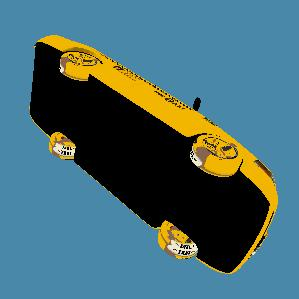
\includegraphics[width=0.4\textwidth]{graphics/taxi.jpg}
    \caption{A render of the taxi model with its original texture. As you can see, the renderer applies parts of the car body texture to the wheels.}
    \label{fig:taxi}
\end{figure}

The original textures of the model had a resolution of 1024x1024, 2048x2048 or 4096x496 pixels. Since the generator requires a each input texture to have the same size, the 4096x4096 textures were downsampled to 2048x2048 using OpenCV's resize function with INTER\_AREA interpolation \footnote{https://learnopencv.com/image-resizing-with-opencv/}. The 1024x1024 pixels textures were upsampled to 2048x2048 pixels using OpenCV's resize function with bicubic interpolation.

Some models have multiple correct labels for two reasons. The first one is that a pre-trained InceptionV3 \cite{inceptionv3} model consistently misclassifies some rendered objects with the same wrong labels, but those labels are semantically related to the correct class. For example, the purse model is often confused with a wallet, but since both a purse and a wallet are made of the same material and have similar colours, we consider this to be meaningful. Similarly, the jeep model is frequently misclassified as a "half-track" and as an "amphibious vehicle", both of those being somewhat similar to jeeps. Secondly, some 3D models can fit in a variety of Imagenet classes. The model of a muscle car can be reasonably described as both a "sports car" and a "race car".

\begin{table}
\caption{The 3D model dataset, with the correct labels of each model, and the classification accuracy of InceptionV3 on rendered images of those models.}
\label{table:model_labels_accuracy}
\begin{tabular}{|p{2.6cm} | p{8.5cm}| p{2cm}|} 
 \hline
 Model Name & Labels & Classification Accuracy (\%) \\
 \hline
 barrel & barrel/cask (427) & 92.8 \\ 
 \hline
 baseball & baseball (429) & 100 \\
 \hline
 camaro & station wagon (436), race car (751), sports car (817) & 10.8 \\
 \hline
 clownfish & anemone fish (393) & 37.2 \\
 \hline
 crocodile & African crocodile (49), American alligator (50) & \\
 \hline
 german\_shepherd & All 118 dog breeds (labels 151 to 268), as well as grey wolf, white wolf, red wolf, coyote, dingo, dhole, hyena dog (labels 269 to 275) & 73.2 \\
 \hline
 jeep & amphibious vehicle (408), half-track (586), jeep (609) & \\
 \hline
 orange & orange (950) & 59 \\
 \hline
 orca & orca (148) & \\
 \hline
 purse & purse (748), wallet (893) & 71 \\
 \hline
 rugby\_ball & rugby ball (768) & \\
 \hline
 running\_shoe & running shoe (770) & \\
 \hline
 sea\_turtle & loggerhead turtle (33), leatherback turtle (34), mud turtle (35), terrapin (36), box turtle (37) & 89.8 \\
 \hline
 taxi & taxi (468) & 15 \\
 \hline
 teddy & teddy bear (850) & 54 \\
 \hline
\end{tabular}
\end{table}


\section{EOT for rendererd 3D objects}

\subsection{Experiment Design}
    \label{subsec:eot_experiment_design}

To validate that our implementation of EOT is correct, we evaluate if the attack success rate is the same as Athalye \textit{et al.} \cite{athalye} reported on their experiments with adversarial examples for 3D rendered objects. For each 3D model, Athalye \textit{et al.} chose 20 random target labels and used EOT to create adversarial textures. Then for each of these 200 textures, they sampled 100 different random poses and rendered images of the 3D model in that pose and with the adversarial texture. These images were fed into Tensorflow's pre-trained InceptionV3 classifier neural network, and the authors measured how often they were classified with the correct label versus the adversarial label.

The procedure used by me is similar. I use 10 out of the 15 models in the dataset, the ones matching the models used by Athalye \textit{et al.}, and for each one 5 target labels are sampled from a uniform distribution, ensuring that they are different to the correct labels. Only 5 target labels are used instead of 20 due to computational and time constraints.

The EOT implementation described in section \ref{sec:eot_implementation} is used to create 50 adversarial textures.  Tensorflow Keras's pre-trained InceptionV3 neural network is used again to evaluate rendered images of the adversarial objects. The algorithm is run until the average loss of the past 400 steps is below 0.5, or for 10000 steps at most. A constant learning rate of 0.003 is used. 

Just as it was done in \cite{athalye}, 80\% of samples from the current mini-batch are re-used in the next mini-batch. For models whose original texture was 1024x1024, I chose to use that rather than the texture upscaled to 2048x2048 pixels, as a smaller texture allows for a larger batch sizes, which gives better results. The batch size is 40 for models with 1024x1024 textures, the same batch size used in \cite{athalye}. For textures with 2048x2048 pixels, the batch size is 30, the maximum that 8GB of memory can fit. 

The authors of \cite{athalye} say that for each model/target label pair they tried four values for the $\lambda$ hyper-parameter from equation \ref{eq:eot} on page \pageref{eq:eot}, used for constraining perceptual difference between normal and adversarial images. They then chose the adversarial example that had the best attack success rate. They do not say what value they used for each adversarial example. Due to time and computation constraints, it was unfeasible to try 4 different $\lambda$ values for each of the 50 adversarial examples. Some ad-hoc experiments done with the crocodile 3D model indicates that a value of 0.025 ensures that the adversarial texture looks similar to the original one, while not still having a high attack success rate. Therefore, this was used for the EOT implementation evaluation.

The rendering parameters are sampled from uniform distributions identical with those used by Athalye \textit{et al.} \cite{athalye}, which you can see in table 2 of their supplementary material. Translation on the X/Y axes is quit small, between -0.05 and 0.05. The rotation angle on all three axes is drawn from an unbounded uniform distribution. The camera distance is between 1.8 and 2.3, while in \cite{athalye} it was between 2.5 and 3. The reason behind this is that the 3D models in my dataset appear to be smaller than those used in \cite{athalye}, and so the camera distance was reduced to make them appear to the camera as large as they did in Athalye \textit{et al.}. You can see in figure \ref{fig:barrel_comparison} that with the adjusted camera distance, the barrel model appears roughly as large as the model used in \cite{athalye}. Finally, because this experiment is on evaluating EOT on 3D rendered objects and not physical 3D printed adversarial objects, printer and camera errors are not modelled, and the apply\_print\_error and apply\_photo\_error functions from algorithm \ref{alg:rendering} on page \pageref{alg:rendering} are not called.

\begin{figure}[H]
\centering
\subfloat[Model used in \cite{athalye}.]{
	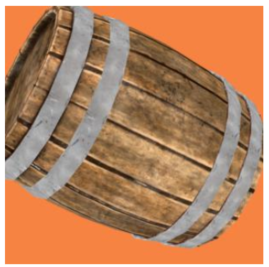
\includegraphics[width=0.4\linewidth]{./graphics/athalye_barrel.png}
}~ % Use a tilde to add spacing for sub-figures that are displayed next to one another horizontally.
\subfloat[Model used by this project.]{
	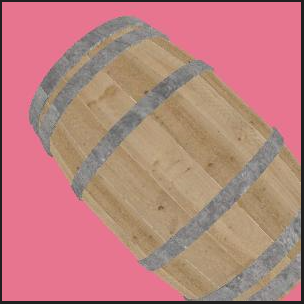
\includegraphics[width=0.4\linewidth]{./graphics/my_barrel.png}
}\\ % New line before caption.

\caption[Comparison of the camera distances used in Athalye \textit{et al.} versus this project.]{A comparison of an image of the barrel model used in Athalye \textit{et al.} versus an image of the barrel model used by this project.}
\label{fig:barrel_comparison}
\end{figure}

After creating the 50 adversarial textures, the same renderer used during the EOT optimisation process is used to create the evaluation images. For each adversarial texture, 100 images of the rendered object with that texture are created. For each image with the adversarial texture, an image of the object in the same pose and with the same background colour, but with the normal texture, is rendered. You can see an example of this in figure \ref{fig:evaluation_images_comparison}. This is done to observe the effect of using the adversarial texture rather than the original one, as all other factors are the same.

\begin{figure}[H]
\centering
\subfloat[Adversarial image.]{
	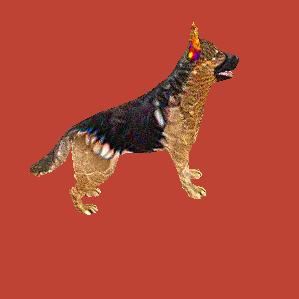
\includegraphics[width=0.485\linewidth]{./graphics/adv_dog_image.jpg}
}~ % Use a tilde to add spacing for sub-figures that are displayed next to one another horizontally.
\subfloat[Normal image.]{
	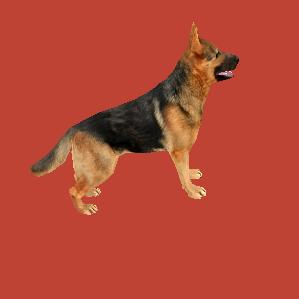
\includegraphics[width=0.485\linewidth]{./graphics/std_dog_image.jpg}
}\\ % New line before caption.

\caption[Comparison between equivalent adversarial and normal images for evaluation.]{Comparison between an evaluation image of the dog model with the adversarial texture versus its normal counterpart. The adversarial texture is for the "black grouse" target label.}
\label{fig:evaluation_images_comparison}
\end{figure}

\subsection{Experiment Results}

On the 5000 images with the normal textures, the average classification accuracy was 60.28\%, while only 0.08\% of them were classified as the adversarial target label. By comparison, the 20000 normal images in Athalye \textit{et al.} \cite{athalye} had an accuracy of 68.8\% and only 0.01\% were classified as the target label. These figures are similar, although my images had a significantly lower classification accuracy. This is caused by the low classification accuracies for normal images of the taxi and camaro models being only 15 and 10.8, as you can see in table \ref{table:model_labels_accuracy}. Without these two models, the average accuracy would be 72.125\%. 

But on the adversarial images, the average classification accuracy was just 0.86\%, very close to the EOT paper's result of 1.1\% \cite{athalye}. Meanwhile, the average TFR was 80.08\%, slightly under the TFR of 83.4\% seen in the EOT paper. The slightly worse performance may be caused by a multitude of factors. Even though the dataset described in section \ref{sec:dataset} is designed to mimick the one used in \cite{athalye}, it is not identical. Furthermore, different values for the $\lambda$ penalty constant, learning rate, and number of steps were used compared to \cite{athalye}, as the authors did not specify what values they used. The mean TFR and the target labels for each individual model can be seen in table\ref{table:eot_results}.

The fact that the adversarial textures brought down the classification accuracy from 60.28\% to 0.86\%, and increased the TFR from 0.08\% to 80.08\%, demonstrates the this implementation of EOT \footnote{https://github.com/Alexandru-Dascalu/adversarial-3d} is highly effective at creating robust adversarial attacks for 3D rendered objects. Moreover, the results are very similar to those in \cite{athalye}, demonstrating that it is an accurate re-creation of the implementation used by the authors of that paper.

All 50 adversarial textures created by and used in this experiment can be seen in appendix \ref{app:adversarial_textures}.

\begin{table}
\caption{Results of the EOT experiment on rendered 3D objects.}
\label{table:eot_results}
\begin{tabular}{|p{2.6cm} | p{6.5cm} | p{2cm}| p{2cm}|} 
 \hline
 Model Name & Target Labels & Mean TFR (\%) & Mean number of iterations \\
 \hline
 barrel & file cabinet, hourglass,hautboy, purse, typewriter keyboard & 95.59 & 1428.4 \\ 
 \hline
 baseball & australian terrier, dingo, indian elephant, radiator, warplane & 80.6 & 6349.2 \\
 \hline
 camaro & kite, mongoose, indri, trombone, red-breasted merganser & 93.39 & 2585.8 \\
 \hline
 clownfish & swimming cap, grand piano, shopping basket, wall clock, bridegroom & 48.2 & 10000 \\
 \hline
 german\_shepherd & bald eagle, barrel, bikini, black grouse, hornbill & 85.6 & 5243 \\
 \hline
 orange & whippet, goblet, lighter, missile, plate & 97.4 & 1163.2 \\
 \hline
 purse & pit bull terrier, chickadee, dhole, weevil, sandbar & 42.8 & 9090.6 \\
 \hline
 sea\_turtle & Australian terrier, leopard, mantis, cradle, plunger & 80.39 & 5123 \\
 \hline
 taxi & groenendael, marmot, acoustic guitar, cradle, radiator grille & 87.8 & 4229.6 \\
 \hline
 teddy & soft-coated wheaten terrier, leatherback turtle, pool table, hot pot, pineapple & 89 & 2782.8 \\
 \hline
\end{tabular}
\end{table}

\subsection{Discussion}

Furthermore, in figure \ref{fig:eot_histogram} you can see a histogram of the TFR for each of the 50 adversarial textures.

\begin{figure}[ht]
    \centering
    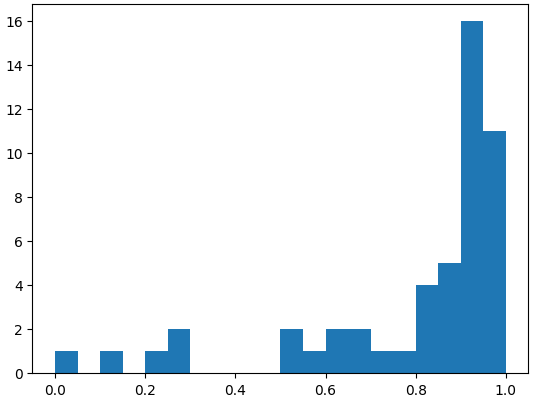
\includegraphics[width=0.7\textwidth]{graphics/eot_histogram.PNG}
    \caption{Histogram of TFR of the 50 adversarial examples.}
    \label{fig:eot_histogram}
\end{figure}

\subsubsection{Classification accuracy on normal images}

The very low InceptionV3 classification accuracies for normal texture images of the taxi and camaro models of 15 and 10.8 percent, respectively, might be caused by the fact that the objects are rendered with completely random rotations on the X, Y and Z axes. Therefore, these cars are often seen from below or above. The images of taxis or sports cars in the Imagenet dataset are of cars as they appear on the street, and therefore seen from the side or from the front or back, not from above or underneath.

Then again, the classification accuracy on images with the nomal texture does not seem to impact the performance of EOT. The adversarial textures for taxi and camaro models had a mean TFR of 87.8\% and 93.39\%, respectively.

\section{G-EOT}

\subsection{Experiment Design}

\subsection{Experiment Results}
    \label{sec:experiment_design}
    
\subsection{Discussion}
